\documentclass{beamer}
\usepackage{hyperref}
\usepackage[T1]{fontenc}
\usepackage{latexsym,amsmath,xcolor,multicol,booktabs,calligra}
\usepackage{graphicx,listings,stackengine}
\usepackage{tcolorbox} 
\usepackage{tikz}
\newcommand{\btext}[1]{\textbf{#1}}
\usetikzlibrary{positioning, arrows.meta, shapes.geometric, fit, backgrounds, calc}
\usepackage{fontawesome5}
\author{Julia Kim \and Xander Backus}
\title{EgoBlind-RA}
\subtitle{Risk-Adaptive Egocentric Visual Assistance for Blind Users}
\institute{
    MAS.S60 \\
}
\date{May 12, 2026}
\usepackage{Ritsumeikan}
\AtBeginSection{}
\AtBeginSubsection{}

\begin{document}

\begin{frame}
    \titlepage
    \vspace*{-0.6cm}
    \begin{figure}[htpb]
        \begin{center}
            \includegraphics[keepaspectratio, scale=0.05]{mit.png}
        \end{center}
    \end{figure}
\end{frame}

%% ============================================================
%% SLIDE 1: Problem & Motivation
%% ============================================================
\section{Problem}
\begin{frame}{Why Urgency Matters for Blind Users}
    \begin{itemize}[<+->]
        \item \textbf{253M} people worldwide live with visual impairment
        \item AI assistants interpret their surroundings via \textbf{egocentric video}
        \begin{center}
        \includegraphics[width=0.8\textwidth]{pic/Screenshot 2026-05-11 at 7.11.30 PM.png}
    \end{center}
        \item Benchmarks (EgoBlind, VizWiz) + VLMs (LLaVA, Kimi-VL) apply a \textbf{uniform policy} to all queries
\end{itemize}
\end{frame}

\begin{frame}{Why Urgency Matters for Blind Users}
\begin{center}

\begin{tabular}{cc}
    \multicolumn{1}{c}{{\textbf{fast, brief answer}}} &
    \multicolumn{1}{c}{\textbf{detailed answer}} \\
    
    \begin{minipage}[t][2.8cm][c]{0.42\textwidth}
        \centering
        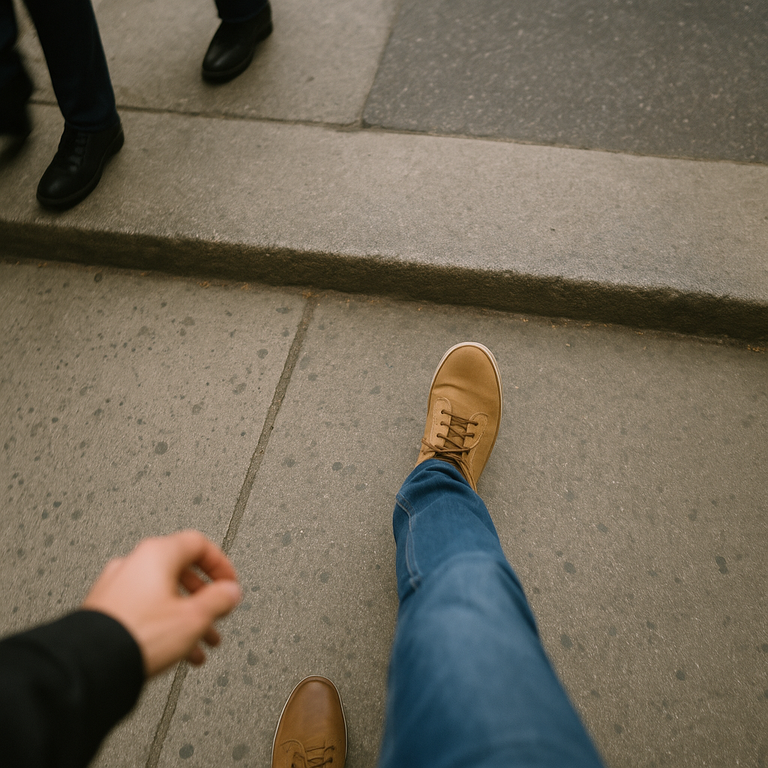
\includegraphics[width=2.5cm, height=2.5cm, keepaspectratio]{pic/step.png}
    \end{minipage}
    &
    \begin{minipage}[t][2.8cm][c]{0.3\textwidth}
        \centering
        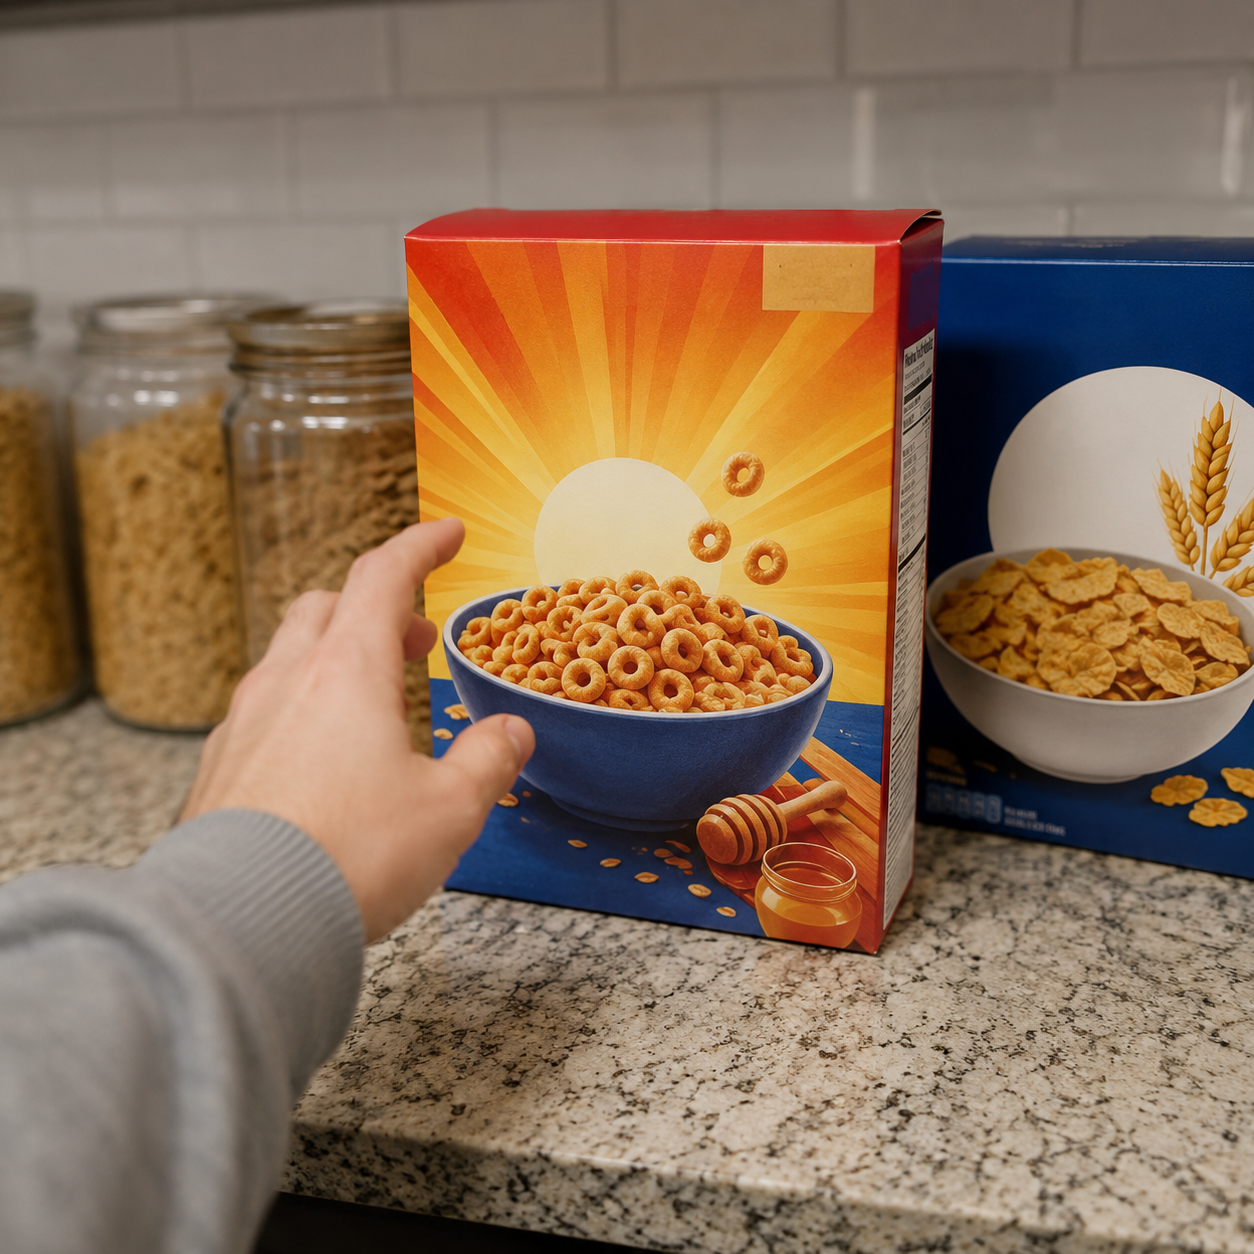
\includegraphics[width=2.5cm, height=2.5cm, keepaspectratio]{pic/cereal.png}
    \end{minipage} \\[-0.5em]
    
    \begin{minipage}[t]{0.42\textwidth}
        \centering
        {\scriptsize \textit{``Is a step in front of me?''}}
    \end{minipage}
    &
    \begin{minipage}[t]{0.42\textwidth}
        \centering
        {\scriptsize \textit{``What cereal brand is this?''}}
    \end{minipage} \\
    
    \begin{minipage}[t][2.8cm][c]{0.42\textwidth}
        \centering
        \includegraphics[width=2.5cm, height=2.5cm, keepaspectratio]{pic/subway.png}
    \end{minipage}
    &
    \begin{minipage}[t][2.8cm][c]{0.42\textwidth}
        \centering
        \includegraphics[width=2.5cm, height=2.5cm, keepaspectratio]{pic/livingroom.png}
    \end{minipage} \\[-0.4em]
    
    \begin{minipage}[t]{0.42\textwidth}
        \centering
        {\scriptsize \textit{``Is anything in my way?''}}
    \end{minipage}
    &
    \begin{minipage}[t]{0.42\textwidth}
        \centering
        {\scriptsize \textit{``Is anything in my way?''}}
    \end{minipage}
\end{tabular}

\end{center}
\end{frame}

\begin{frame}{Our Goal}
\vfill
\begin{tcolorbox}[
    colback=ritsumeikan!5,
    colframe=ritsumeikan,
    arc=4mm,
    boxrule=0.8pt,
    left=14pt, right=14pt, top=14pt, bottom=14pt
]
\large
\textbf{Our goal:} classify query urgency from video + text, \textit{then} route to a response calibrated to the safety stakes.
\end{tcolorbox}
\vfill
\end{frame}

%% ============================================================
%% SLIDE 2: Method
%% ============================================================
\section{Method}
\begin{frame}{Stage 1: CLIP Urgency Classifier}
\begin{center}
\footnotesize
\textcolor{ritsumeikan}{\boldmath\textbf{$\text{urgency} = \text{MLP}\big(\text{mean-pool}(\text{CLIP}_v(\text{frames})) \oplus \text{CLIP}_t(\text{question})\big)$}}
\end{center}
\begin{center}
\resizebox{\textwidth}{!}{%
\begin{tikzpicture}[
    node distance=0.6cm,
    every node/.style={align=center, font=\footnotesize},
    input/.style={draw, rounded corners, thick, fill=gray!10, minimum width=1.7cm, minimum height=0.7cm},
    encoder/.style={draw, rounded corners, thick, fill=ritsumeikan!15, minimum width=1.9cm, minimum height=0.7cm},
    op/.style={draw, circle, thick, fill=gray!5, minimum size=0.5cm, inner sep=0pt},
    head/.style={draw, rounded corners, thick, fill=ritsumeikan!30, minimum width=1.7cm, minimum height=0.7cm},
    output/.style={draw, rounded corners, thick, fill=ritsumeikan, text=white, minimum width=1.7cm, minimum height=0.7cm},
    arrow/.style={->, thick, >=stealth}
]
    \node[input] (frames) {4 video \\ frames};
    \node[input, below=1cm of frames] (text) {Question \\ text};
    \node[encoder, right=0.7cm of frames] (vis) {CLIP ViT-B/32 \\ \scriptsize (frozen)};
    \node[encoder, right=0.7cm of text] (txt) {CLIP text enc. \\ \scriptsize (frozen)};
    \node[op, right=0.6cm of vis] (pool) {$\bar{\mu}$};
    \node[op, right=1.1cm of pool, yshift=-0.85cm] (concat) {$\oplus$};
    \node[head, right=0.6cm of concat] (mlp) {2-layer MLP \\ \scriptsize (BCE)};
    \node[output, right=0.6cm of mlp] (out) {Urgency \\ score};
    \draw[arrow] (frames) -- (vis);
    \draw[arrow] (text) -- (txt);
    \draw[arrow] (vis) -- (pool);
    \draw[arrow] (pool) -| (concat);
    \draw[arrow] (txt) -| (concat);
    \draw[arrow] (concat) -- (mlp);
    \draw[arrow] (mlp) -- (out);
    \node[below=0.05cm of pool, font=\scriptsize\itshape] {mean-pool};
    \node[above=0.05cm of concat, font=\scriptsize\itshape] {concat};
\end{tikzpicture}%
}
\end{center}
\vfill 
\begin{itemize}
    \item Test ROC-AUC: \textbf{0.905} $\to$ strong signal from frozen features
\end{itemize}
\end{frame}\begin{frame}{Stage 2: Two Architectural Approaches}
\begin{center}
\resizebox{!}{0.85\textheight}{%
\begin{tikzpicture}[
    every node/.style={align=center, font=\footnotesize},
    input/.style={draw=gray!60, rounded corners, thick, fill=gray!15, minimum width=4cm, minimum height=1cm},
    classifier/.style={draw=ritsumeikan, rounded corners, thick, fill=ritsumeikan!12, minimum width=4.4cm, minimum height=1cm},
    score/.style={draw=ritsumeikan, rounded corners=10pt, thick, fill=ritsumeikan!12, minimum width=3.6cm, minimum height=0.9cm},
    decision/.style={draw=gray!60, diamond, thick, fill=gray!15, aspect=2, inner sep=1pt, minimum width=1.5cm},
    urgent/.style={draw=ritsumeikan, rounded corners, thick, fill=ritsumeikan!55, text=white, minimum width=2cm, minimum height=0.95cm},
    nonurg/.style={draw=ritsumeikan, rounded corners, thick, fill=ritsumeikan!15, minimum width=2cm, minimum height=0.95cm},
    tag/.style={draw=ritsumeikan, rounded corners, thick, fill=ritsumeikan!28, minimum width=3.2cm, minimum height=1cm},
    unified/.style={draw=ritsumeikan, rounded corners, thick, fill=ritsumeikan!28, minimum width=3.2cm, minimum height=1cm},
    response/.style={draw=gray!60, rounded corners, thick, fill=gray!15, minimum width=4cm, minimum height=1cm},
    container/.style={draw=gray!70, dashed, rounded corners, thick, inner sep=14pt},
    arrow/.style={->, thick, >=stealth, gray!50!black}
]
    % Shared top
    \node[input] (input) at (0,0) {\textbf{Input} \\ \footnotesize Video frames + question};
    \node[classifier] (clip) at (0,-1.6) {\textbf{Stage 1: CLIP classifier} \\ \footnotesize Frozen ViT-B/32 + MLP head};
    \node[score] (score) at (0,-3.2) {$\hat{u} \in \{\text{urgent, not}\}$};

    % Approach 1
    \node[decision] (diamond) at (-4, -5.5) {$\hat{u}$?};
    \node[urgent] (urg1) at (-5.2, -7.3) {\textbf{Urgent} \\ \footnotesize SFT adapter};
    \node[nonurg] (nu1) at (-2.8, -7.3) {\textbf{Non-urgent} \\ \footnotesize SFT+DPO};

    % Approach 2
    \node[tag] (tag2) at (4, -5.5) {\textbf{Prepend tag} \\ \footnotesize [URGENT] / [NON-URG]};
    \node[unified] (uni2) at (4, -7.3) {\textbf{Unified adapter} \\ \footnotesize Single SFT LoRA};

    % Response
    \node[response] (resp) at (0, -10) {\textbf{Response} \\ \footnotesize Urgency-calibrated answer};
    \node[below=0.05cm of resp, font=\scriptsize, gray!60!black] {Base model: Kimi-VL-A3B-Instruct};

    % Containers (background)
    \begin{scope}[on background layer]
        \node[container, fit=(diamond)(urg1)(nu1)] (cont1) {};
        \node[container, fit=(tag2)(uni2)] (cont2) {};
    \end{scope}
    \node[font=\footnotesize, gray!50!black, anchor=north west] 
        at ([xshift=30pt, yshift=-2pt]cont1.north west) {Approach 1: bifurcated};
    \node[font=\footnotesize, gray!50!black, anchor=north west] 
        at ([xshift=30pt, yshift=-2pt]cont2.north west) {Approach 2: unified};

    % Arrows
    \draw[arrow] (input) -- (clip);
    \draw[arrow] (clip) -- (score);
    \draw[arrow] (score.south) -- ++(0,-0.3) -| ([xshift=15pt]cont1.north);
    \draw[arrow] (score.south) -- ++(0,-0.3) -| ([xshift=15pt]cont2.north);
    \draw[arrow] (diamond.south) -- node[left, font=\scriptsize, pos=0.5] {1} (urg1.north);
    \draw[arrow] (diamond.south) -- node[right, font=\scriptsize, pos=0.5] {0} (nu1.north);
    \draw[arrow] (tag2) -- (uni2);
    \coordinate (m1) at (-4, -8.7);
    \draw[gray!50!black, thick] (urg1.south) |- (m1);
    \draw[gray!50!black, thick] (nu1.south) |- (m1);
    \draw[arrow] (m1) |- (resp.west);
    \draw[arrow] (uni2.south) |- (resp.east);
\end{tikzpicture}%
}
\end{center}
\end{frame}

%% ============================================================
%% SLIDE 3: SFT Results
%% ============================================================
\section{Results}
\begin{frame}{SFT Dramatically Improves Over Baseline}
\footnotesize
For each $(v, q)$, the model learns to mimic a length-calibrated reference answer.
\begin{center}
\begin{tabular}{cc}
    \begin{minipage}{0.42\textwidth}
        \centering
        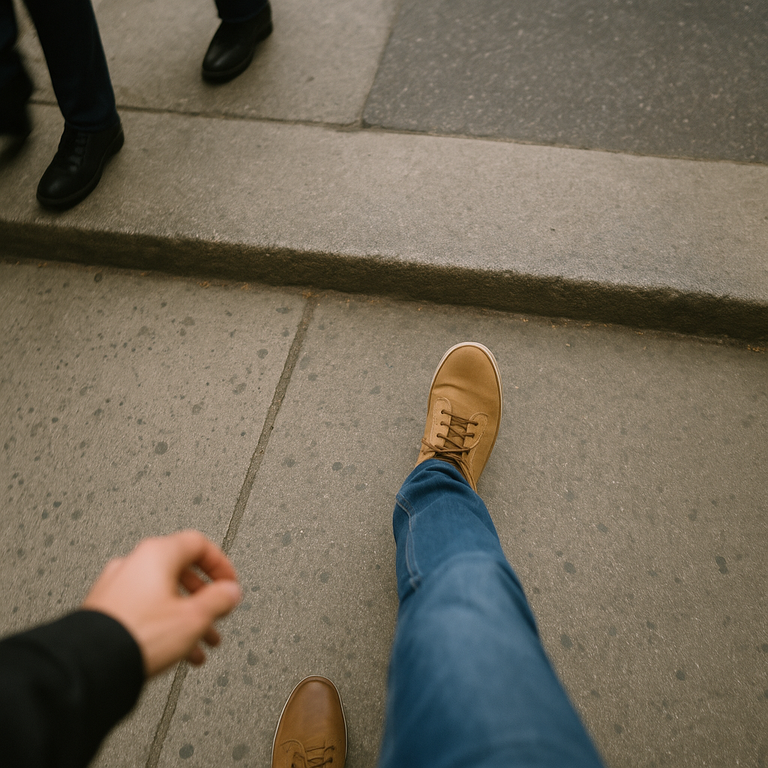
\includegraphics[width=0.5\textwidth]{pic/step.png} \\[0.3em]
        {\scriptsize \textit{``Is a step in front of me?''}} \\[0.2em]
        {\scriptsize \textbf{shortest} ref: \textit{``Yes, step.''}}
    \end{minipage}
    &
    \begin{minipage}{0.42\textwidth}
        \centering
        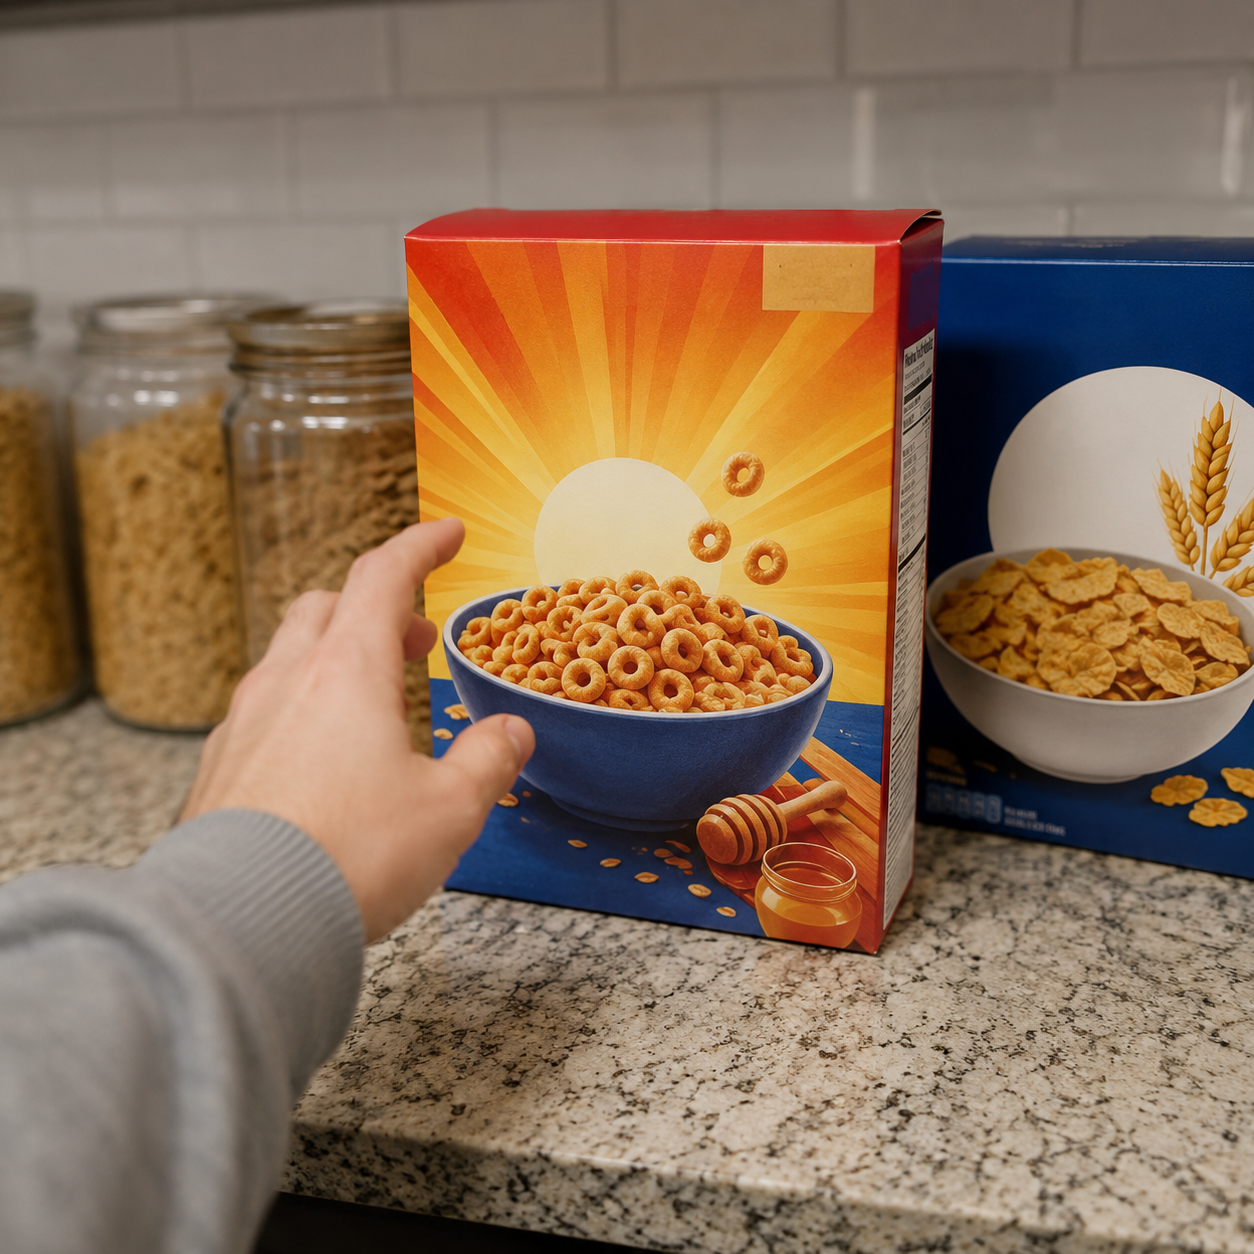
\includegraphics[width=0.5\textwidth]{pic/cereal.png} \\[0.3em]
        {\scriptsize \textit{``What cereal brand is this?''}} \\[0.2em]
        {\scriptsize \textbf{longest} ref: \textit{``Honey Bunches of Oats...''}}
    \end{minipage}
\end{tabular}
\end{center}

\vspace{0.2em}
\begin{table}
    \centering
    \small
    \begin{tabular}{lccc}
        \toprule
        & \textbf{Loss $\downarrow$} & \textbf{Similarity $\uparrow$} & \textbf{Mean words} \\
        \midrule
        Baseline (uniform policy) & 0.607 & 0.350 & 84.1 \\
        Approach 1 & 0.556 & 0.393 & 4.5 \\
        Approach 2 & \textbf{0.375} & \textbf{0.589} & 2.2 \\
        \bottomrule
    \end{tabular}
\end{table}
\end{frame}
\begin{frame}{Key SFT Discoveries}
\begin{itemize}
    \item \textbf{Vision conditioning is essential:} text-only training collapses to ``Yes''/``No'' for 71\% of urgent queries

    \pause
    
    \item \textbf{Light LoRA prevents overfitting:} rank 8, \texttt{q\_proj} + \texttt{v\_proj}, 1 epoch (vs.\ rank 16, all projections, 5+ epochs)
\end{itemize}
\end{frame}


%% ============================================================
%% SLIDE 4: DPO --- the surprising finding
%% ============================================================
\begin{frame}{DPO: Architecture Determines Whether It Helps}
\footnotesize
For each $(q, v)$, DPO sees two candidate responses and learns to prefer the better one. 
\vspace{0.4em}

\begin{tabular}{cc}
    \begin{minipage}{0.3\textwidth}
    \centering
    \vspace{0.5cm}
    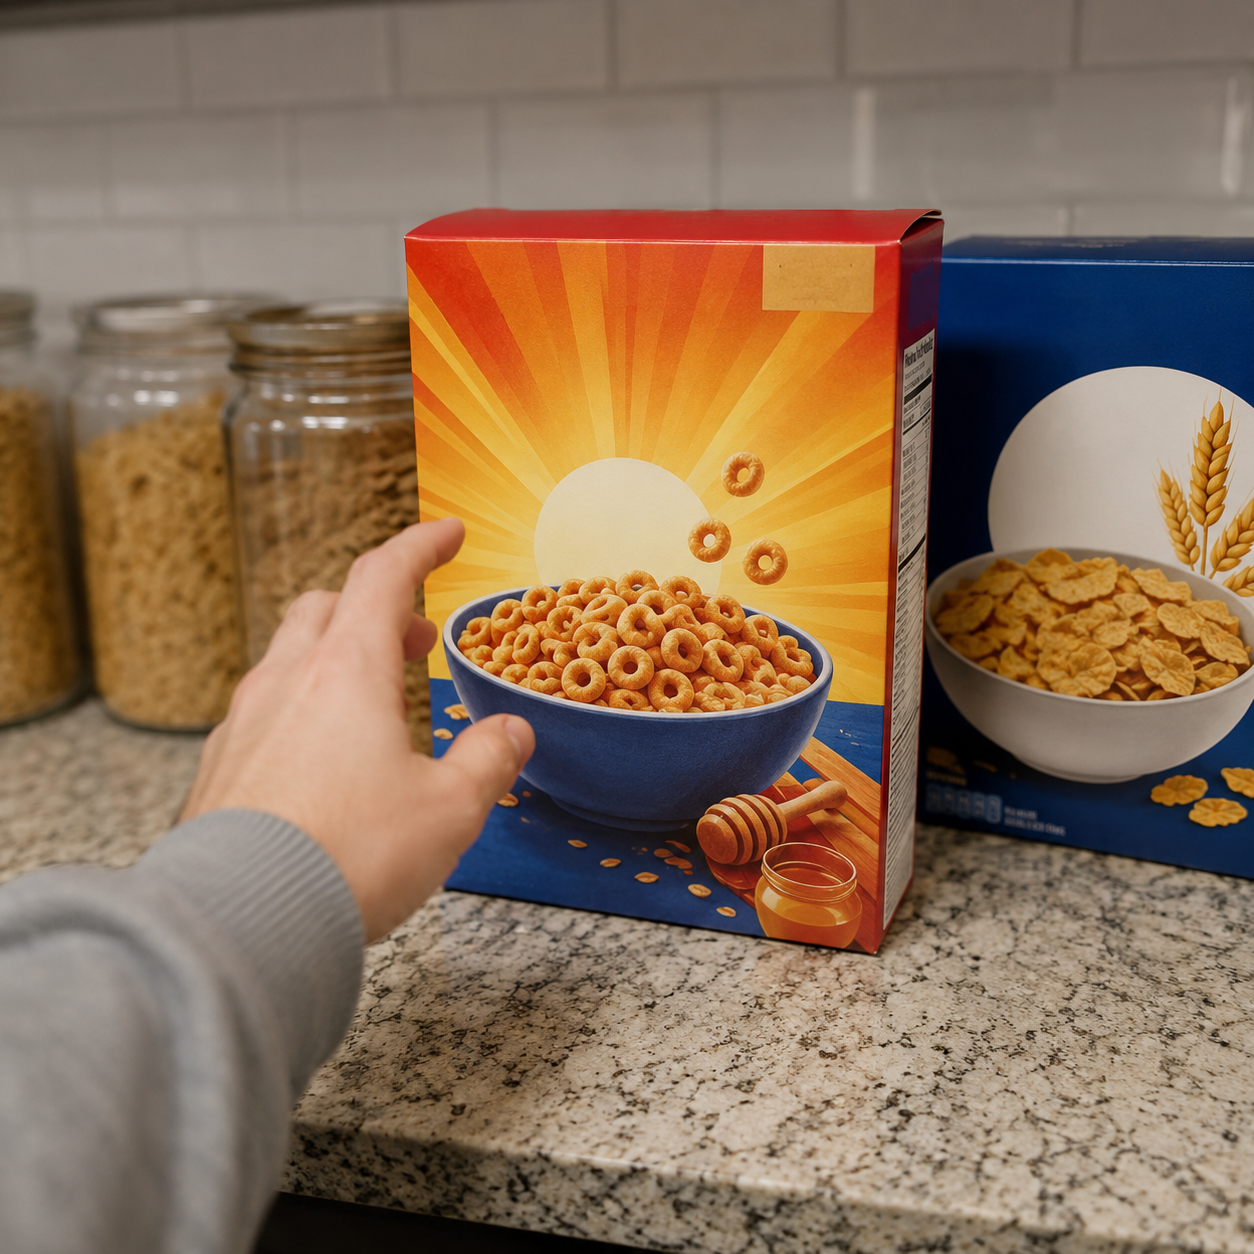
\includegraphics[width=0.7\textwidth]{pic/cereal.png} \\[0.3em]
    {\scriptsize \textit{``What cereal brand is this?''}}
\end{minipage}
    &
    \begin{minipage}{0.55\textwidth}
        \begin{tcolorbox}[colback=green!8, colframe=green!50!black, arc=2mm, boxrule=0.6pt, left=6pt, right=6pt, top=4pt, bottom=4pt]
        \scriptsize
        \textcolor{green!50!black}{\textbf{Chosen}} \\
        \textit{``Honey Bunches of Oats, on the counter next to a bowl.''}
        \end{tcolorbox}
        \begin{tcolorbox}[colback=red!8, colframe=red!50!black, arc=2mm, boxrule=0.6pt, left=6pt, right=6pt, top=4pt, bottom=4pt]
        \scriptsize
        \textcolor{red!50!black}{\textbf{Rejected}} \\
        \textit{``Cereal.''}
        \end{tcolorbox}
    \end{minipage}
\end{tabular}

\vspace{1.3em}
\begin{columns}[T]
    \begin{column}{0.48\textwidth}
        \centering
        \textbf{Approach 2 (unified)} \\
        \footnotesize \textcolor{red!70!black}{DPO regresses SFT}
        \vspace{0.3em}
        
        \scriptsize
        \begin{tabular}{lc}
            \toprule
            \textbf{Method} & \textbf{Loss $\downarrow$} \\
            \midrule
            SFT & \textbf{0.375} \\
            SFT $\to$ DPO & \textcolor{red!70!black}{0.433} \\
            \bottomrule
        \end{tabular}
    \end{column}
    \pause
    \begin{column}{0.48\textwidth}
        \centering
        \textbf{Approach 1 (bifurcated)} \\
        \footnotesize \textcolor{red!70!black}{hurts urgent}, \textcolor{green!50!black}{helps non-urgent}
        \vspace{0.3em}
        
        \scriptsize
        \begin{tabular}{lcc}
            \toprule
            & \textbf{Urgent} & \textbf{Non-urg.} \\
            \midrule
            SFT & \textbf{0.505} & 0.268 \\
            SFT+DPO & \textcolor{red!70!black}{0.459} & \textcolor{green!50!black}{\textbf{0.298}} \\
            \bottomrule
        \end{tabular}
    \end{column}
\end{columns} 
\end{frame} 


%% ============================================================
%% SLIDE 5: Pipeline + Conclusion
%% ============================================================
\section{Conclusion}
\begin{frame}{End-to-End Pipeline} 
\begin{center}
{\textcolor{ritsumeikan}{\textbf{How does each architecture handle \textit{real} classifier routing?}}}
\end{center}

\begin{table}
    \centering
    \small
    \begin{tabular}{lcc}
        \toprule
        \textbf{Routing strategy} & \textbf{Approach 1} & \textbf{Approach 2} \\
                                  & \textbf{Loss $\downarrow$} & \textbf{Loss $\downarrow$} \\
        \midrule
        Baseline (no routing)         & 0.607 & 0.607 \\
        \textbf{CLIP classifier (ours)} & \textbf{0.556} & \textbf{0.375} \\
        \textcolor{gray}{Oracle (ground-truth)} & \textcolor{gray}{0.549} & \textcolor{gray}{0.375} \\
        \midrule
        Gap to oracle & 0.007 & \textbf{0.000} \\
        \bottomrule
    \end{tabular}
\end{table}

\begin{tcolorbox}[
    colback=ritsumeikan!5,
    colframe=ritsumeikan,
    arc=4mm,
    boxrule=0.8pt,
    left=8pt, right=8pt, top=6pt, bottom=6pt
]
\footnotesize
For blind users, \textbf{Approach 2 is safer}: misrouted urgent queries still get a competent answer.
\end{tcolorbox}
\end{frame}

%% ============================================================
%% THANK YOU
%% ============================================================
\begin{frame}
\vfill
\begin{center}
    {\Huge\calligra Thank You}

    \vspace{1.5cm}

    \normalsize
    \begin{tabular}{rl}
        \textbf{Code:} & \href{https://github.com/juliavekim/EgoBlind-RA}{github.com/juliavekim/EgoBlind-RA} \\[0.3em]
                       & \href{https://github.com/xabackus/mmai}{github.com/xabackus/mmai} \\[0.6em]
        \textbf{Classifier:} & \href{https://huggingface.co/julia225/egoblind-ra-clip-urgency}{huggingface.co/julia225/egoblind-ra-clip-urgency}
    \end{tabular}
\end{center}
\vfill
\end{frame}

\end{document}